

\begin{table}\centering
\begin{tabular}{|c||c|c|c|}\hline
  Dataset & Nodes & Edges & Comment\\
  \hline Bal. Tree & 40 & 39 & Tree\\
  Phy. Tree & 344 & 343 & Tree\\
  \hline\hline CS PhDs & 1025 & 1043 & Tree-like\\
  WordNet & 74374 & 75834 & Tree-like\\
  \hline\hline Diseases & 516 & 1188 & Dense\\
 Gr-QC & 4158 &  13428& Dense\\
  \hline
\end{tabular}
\caption{Datasets Statistics.}
\end{table}

\begin{table}[h]
\centering
\begin{tabular}{|l||c|c|c|} \hline
Dataset     	          &  C-$\mathbb{H}_2$ &  FB $\mathbb{H}_5$ & FB $\mathbb{H}_{200}$                  \\ \hline\hline
WordNet & 0.989 & 0.823* & 0.87*\\
  \hline
\end{tabular}
\caption{MAP measure for WordNet embedding compared to values in \citet{fb}. Closer to 1 is better.}
\label{table:wordnet_results}
\end{table}

\begin{table}[h]
\centering
\begin{tabular}{|l||c|c||c|c|c|c|c|} \hline
  Dataset     	          &  C-$\mathbb{H}_2$ &  FB $\mathbb{H}_2$ & h-MDS & PyTorch & PWS & PCA & FB                  \\ \hline\hline
  Bal. Tree         & {\bf 0.013}         &      0.425               &    {\bf 0.077}     & 0.034 & 0.020   &  0.496    & 0.236 \\ 
  Phy. Tree          & {\bf 0.006}             &     0.832               &  {\bf   0.039}    & 0.237 & 0.092 &   0.746        &       0.583     \\
\hline \hline
CS PhDs              & {\bf 0.286}    &   0.542                           &  {\bf 0.149}  & 0.298 & 0.187   &  0.708  & 0.336   \\ 
%WordNet              & {\bf 0.054}           &     0.793                &               &  & 0.503\\
\hline\hline 
Diseases              & {\bf 0.147}    &    0.410                          &  0.111  & {\bf 0.080} &  0.108   &    0.595 &  0.764              \\ \hline 
%Gr-QC               & 0.603    &   {\bf 0.387}                               & 0.530    &   0.546 &   0.713\\ \hline 
Gr-QC               & {\bf 0.354}    &   -                               & 0.530  & {\bf 0.125} & 0.134 &   0.546 &   -\\ \hline 

  
\end{tabular}
\caption{Distortion measures using combinatorial and h-MDS techniques, compared against PCA and results from \citet{fb}. Closer to 0 is better.}
\label{table:distortion_results}
\end{table}

\begin{table}[h]
\centering
\begin{tabular}{|l||c|c||c|c|c|c|c|} \hline
  Dataset     	          &  C-$\mathbb{H}_2$ &  FB $\mathbb{H}_2$ & h-MDS & PyTorch & PWS & PCA & FB                  \\ \hline\hline
  Bal. Tree          & {\bf 1.0}              &    0.846    &    {\bf 1.0}    & {\bf 1.0} & {\bf 1.0}       &  {\bf 1.0}           & 0.859     \\ 
Phy. Tree          &      {\bf 1.0}                &    0.718  &   0.675    & 0.951 & 0.998          &    {\bf 1.0}          &       0.811     \\
\hline
\hline
CS PhDs              & {\bf 0.991}             &  0.567          &  0.463    &     0.799 & {\bf 0.945} &              0.541 & 0.78  \\ 
%WordNet              &     {\bf 0.989}            &  0.823$^*$                          &     &            &   0.870 $^*$\\ \hline
\hline\hline
Diseases              &      {\bf 0.822}             & 0.788          &     0.949    &  0.995  &  0.897      &         {\bf 0.999}      &    0.934\\
\hline
%Gr-QC                          &    0.759      &  0.635               &    0.710   &  0.738  &  {\bf 0.999}$^*$  \\ \hline 
Gr-QC                          &    0.696      & -               &    0.710  & 0.733 & 0.504 &  0.738  &  {\bf 0.999}$^*$  \\ \hline 
\end{tabular}
\caption{MAP measures using combinatorial and h-MDS techniques, compared against PCA. %Note results with asterix are from \citet{fb}.
Closer to 1 is better.}
\label{table:map_results}
\end{table}



We evaluate the proposed approaches and compare against
existing methods. We hypothesize that for tree-like data, the
combinatorial construction offers the best performance. For general
data, we expect h-MDS to produce the lowest distortion, while it may
have low MAP due to precision limitations. We anticipate that
dimension is a critical factor (outside of the combinatorial
construction). Finally, we expect that the MAP of h-MDS techniques can
be improved by learning the correct scale and weighting the loss
function as suggested in earlier sections. In the Appendix, we report
on additional datasets, parameters found by the combinatorial
construction, and the effect of hyperparameters.%, and on reducing 
%the precision required by the combinatorial construction by increasing the dimension; 
%as we observed in Section~\ref{sec:combinatorial}, we can reduce the scaling by
%a factor depending on $\operatorname{deg}_{\max}$, but the $\frac{1+\epsilon}{\epsilon}$ term is
%significant.
%For $\varepsilon=1.0$, however, we can store components in 64 bits.

\begin{figure}
\centering
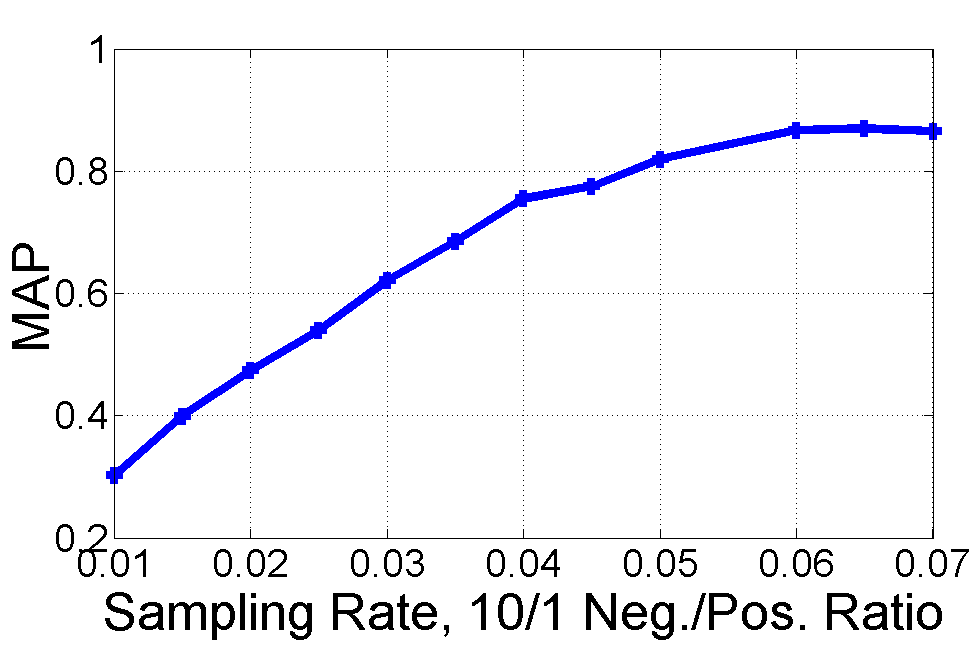
\includegraphics[width=0.4\textwidth]{figures/samplingMAP.png}
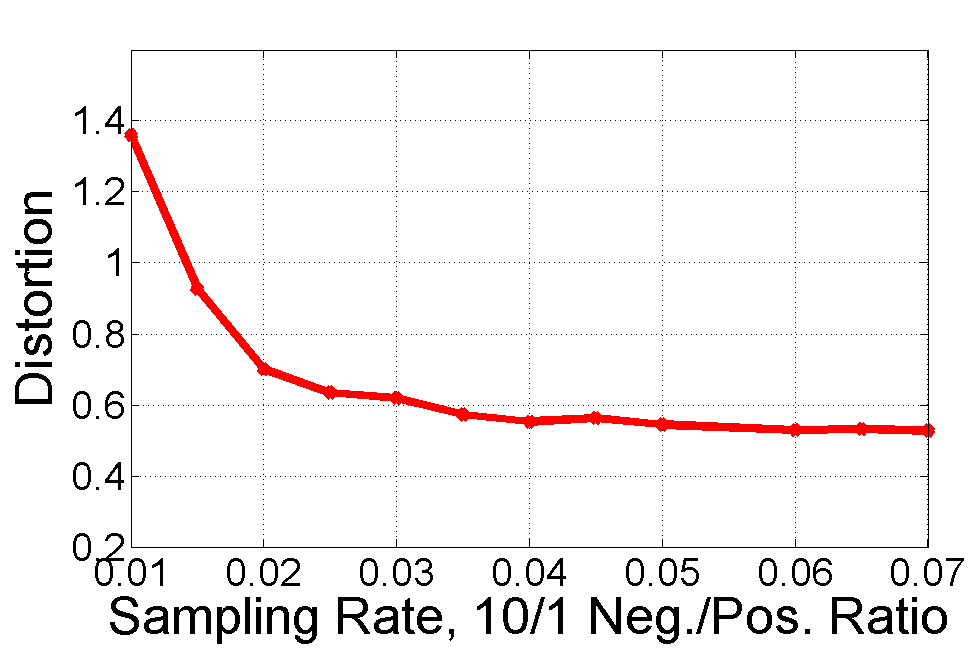
\includegraphics[width=0.4\textwidth]{figures/samplingDistortion.png}
\caption{Learning from incomplete information. The distance matrix is
  sampled, completed, and embedded.}
\label{fig:sampling}
\end{figure}

%\yell{We we are able to deal with
%  incomplete data. Vary amount of data}


\begin{table}[]
\centering
\begin{tabular}{|r||c|c|c|}
\hline 
Rank  & No Scale  &  Learned Scale  &  Exp. Weighting \\    \hline    \hline
50 & 0.481 & 0.508 & {\bf 0.775} \\  \hline
100 & 0.688 & 0.681 & {\bf 0.882}\\ \hline
200 & 0.894 & 0.907 & {\bf 0.963}\\ \hline
\end{tabular}
\caption{Ph.D. dataset. Improved MAP performance of PyTorch implementation using a modified PGA-like loss function.}
\label{table:pytorch}
\end{table}

\paragraph*{Datasets}
We consider trees, tree-like hierarchies, and graphs that are not
tree-like. First, we consider hierarchies that form trees:
fully-balanced trees along with phylogenetic trees expressing genetic
heritage (of mosses growing in urban environments \cite{phylo-tree}, available from \cite{treebase}). Similarly, we used hierarchies that are nearly tree-like:
WordNet hypernym (the largest connected component from~\citet{fb}) and
a graph of Ph.D. advisor-advisee relationships \cite{de2011exploratory}. Also included are
%several
datasets that vary in their tree nearness, such as biological sets
involving disease relationships \cite{goh2007human} and protein interactions in yeast
bacteria \cite{jeong2001lethality}, both available from \cite{nr}. We also include the collaboration network formed by authorship relations for papers submitted to the general relativity and quantum cosmology (Gr-QC) arXiv \cite{grqc}.
%, and a scientific authorship network involving papers
% from the Gr-QC arXiv that were used in prior work.

\paragraph*{Approaches} Combinatorial
embeddings into $\mathbb{H}_2$ are done using Steiner trees generated
from a randomly selected root for the $\varepsilon=0.1$ precision
setting; others are considered in the Appendix. We performed h-MDS in
floating point precision.
We also include results for our PyTorch implementation of an SGD-based algorithm (described later),
as well as a warm start version initialized with the high-dimensional combinatorial construction.
We compare against classical MDS (i.e.,
PCA), and the optimization-based approach~\citet{fb}, which we call
FB. The experiments for h-MDS, PyTorch SGD, PCA, and FB used dimensions of
2,5,10,50,100,200; we recorded the best resulting MAP and
distortion. Due to the large scale, we did not replicate the best FB
numbers on large graphs (i.e., Gr-QC and WordNet).
%(e.g., WordNet).
As a result, we
report their best published MAP numbers for comparison (their work does not report distortion). These entries are marked with an asterisk. For the WordNet
graph we use a random BFS tree rather than a Steiner tree. Moreover, for comparison against FB (which computes the transitive closure), we can use a weighted version of the graph that captures the ancestor relationships. The full details are in Appendix.


\paragraph*{Quality}
In Table~\ref{table:distortion_results}, we report the distortion. As
expected, when the graph is a tree or tree-like the combinatorial
construction has exceedingly low distortion. Because h-MDS is meant to recover
points exactly, we hypothesized that h-MDS would offer very low distortion
on these datasets. We confirm this hypothesis: among h-MDS, PCA, and FB, h-MDS
consistently offers the best (lowest) distortion, producing, for
example, a distortion of $0.039$ on the phylogenetic tree dataset. %We
% see that both PCA and FB have larger distortion, as expected.
We observe that the optimization-based approach works quite well for reducing distortion,
and on tree-like datasets it is bolstered by appropriate initialization from the combinatorial construction.


Table~\ref{table:map_results} reports the MAP measure (this is shown in Table~\ref{table:wordnet_results} for WordNet), which is a
local measure. We expect that the combinatorial construction performs
well for tree-like hierarchies. This is indeed the case: on trees and
tree-like graphs, the MAP is close to 1, improving on approaches such
as FB that rely on optimization. On larger graphs like WordNet, our
approach yields a MAP of $0.989$--improving on the FB MAP result of
$0.870$ at 200 dimensions. This is exciting because the combinatorial
approach is deterministic and linear-time. In addition, it suggests
that this refined understanding of hyperbolic embeddings may be used
to improve the quality and runtime state of the art constructions. As
expected, the MAP of the combinatorial construction decreases as the
graphs are less tree-like.
% However, note that the FB construction
% reports a much better MAP on the Gr-QC dataset ($0.999$) than our
% combinatorial construction $0.759$.
Interestingly, h-MDS solved in
floating point indeed struggles with MAP. We separately confirmed that
it is indeed due to precision using a high-precision solver, which
obtains a perfect MAP---but uses 512 bits of precision. It may be
possible to compensate for this with scaling, but we did not explore
this possibility.


\paragraph*{SGD-Based Algorithm}
We also built an SGD-based algorithm implemented in PyTorch. Here the
loss function is equivalent to the PGA loss, and so is continuously
differentiable. We use this to verify two claims:

\textit{Learned Scale.}
In Table~\ref{table:pytorch}, we verify the importance of scaling that
our analysis suggests; our implementation has a simple learned scale
parameter. Moreover, we added an exponential weighting to the
distances in order to penalize long paths, thus improving the local
reconstruction. These techniques indeed improve the MAP; in
particular, the learned scale provides a better MAP at lower rank. We
hope these techniques can be useful in other embedding techniques.

\textit{Incomplete Information.} 
To evaluate our algorithm's ability to deal with incomplete
information, we examine the quality of recovered solutions as we
sample the distance matrix. We set the sampling rate of non-edges to
edges at $10:1$ following~\citet{fb}. We examine the phylogenetic
tree, which is full rank in Euclidean space. In
Figure~\ref{fig:sampling}, we are able to recover a good solution with a
small fraction of the entries for the phylogenetic tree dataset; for
example, we sampled approximately $4\%$ of the graph but provide a MAP
of $0.74$ and distortion of less than $0.6$. Understanding the sample
complexity for this problem is an interesting theoretical question.



